\documentclass[10pt]{article}
\usepackage{icmlko}

\icmlmeta{IP 파운데이션 월드모델}{10}{굿즈는 건너갔다}{한 축이 처음으로 도메인을 넘었다 --- 순열 p=0.034, 그리고 되돌아오지는 못했다}

\begin{document}

\twocolumn[
\icmlheader

\begin{abstract}
노트 9는 전이 실패의 원인을 축이 아니라 내 매핑으로 지목하고 반증 조건을 적었다 ---
앨범 가격을 굿즈 규모로 옮겼을 때도 부호가 어긋나면 그때는 축 자체가 도메인 특수한
것이다. 옮겼다. 부호 반전이 사라졌다(입장 허들 $-$0.201 대 $+$0.229 $\to$ 축 제거,
남은 셋 중 둘 일치). 그러나 세 축 전체의 전이는 부트스트랩을 붙이자 유의하지 않았다
--- 점추정만 보면 양방향 모두 이겼는데(차이 $-$0.0041과 $-$0.0237) 출처 표본을
다시 뽑으면 부호가 흔들렸다. 축을 하나씩 떼어 보니 이유가 나왔다. \textbf{굿즈 규모
단독으로 팝업에서 아이돌로 보내면 유의하게 이긴다} --- 차이 $-$0.0556, 순열 검정
p=0.034, 부트스트랩 승률 95\%. 이 프로젝트 최초의 도메인 간 전이다. 그런데 두 가지
단서가 붙는다. 첫째, \textbf{되돌아오지 못한다} --- 아이돌에서 팝업으로는 승률 29\%다.
둘째, \textbf{축을 더할수록 희석된다} --- 타깃 폭을 넣으면 승률이 94\%에서 79\%로,
셋을 다 넣으면 64\%로 떨어진다. 전이는 방향이 있고, 그 방향은 잘 측정된 쪽에서
못 측정된 쪽이다. 노트 9의 신뢰도 문턱이 다른 얼굴로 다시 나타났다.
\end{abstract}
]

\section{반증 조건을 실행했다}

노트 9의 마지막 주장 상자는 이랬다.

\begin{quote}\fontsize{9.2}{11}\selectfont
전이 실패의 원인은 축이 도메인 특수해서가 아니라 아이돌 쪽 축 매핑이 틀렸기
때문이다. 앨범 가격은 입장 허들이 아니라 굿즈 규모다.\\[0.3em]
\textbf{반증 조건.} 앨범 가격을 굿즈 규모로 옮기고 입장 허들의 다른 대응물을 넣었을
때도 부호가 어긋나면, 그때는 매핑이 아니라 축 자체가 도메인 특수한 것이다.
\end{quote}

옮겼다. 굿즈 규모를 버전 수와 정가의 가중 결합으로 다시 정의하고, 입장 허들은
대응물이 없으므로 비웠다 --- 팬클럽 가입 비용이나 예약 경쟁 구조 같은 진짜 진입
비용은 아직 수집하지 않았다. 남은 세 축(타깃 폭, 미디어 투입, 굿즈 규모)으로
다시 쟀다.

\begin{table}[t]
\centering\tsize
\caption{매핑 수정 후. 팝업 75건, 아이돌 63건(세 축 완전 케이스).}
\begin{tabular}{lrrl}
\toprule
축 & 팝업 & 아이돌 & \\
\midrule
미디어 투입 & $+$0.126 & $+$0.206 & 일치 \\
굿즈 규모   & $+$0.156 & $+$0.388 & 일치 \\
타깃 폭     & $+$0.310 & $-$0.011 & 아이돌에서 무효 \\
\bottomrule
\end{tabular}
\end{table}

부호 반전은 사라졌다. 남은 불일치는 타깃 폭 하나이며, 그것은 반전이 아니라
아이돌에서 사실상 0이다 --- 인원 수·성별·서바이벌 출신으로 만든 대리변수가 팝업의
``대상이 얼마나 넓은가''와 같은 것을 재지 않는다.

\section{점추정은 이겼고 부트스트랩은 아니었다}

세 축으로 교차 검정하니 양방향 모두 점추정이 음수였다.

\begin{table}[t]
\centering\tsize
\caption{세 축 교차 검정. 부트스트랩은 출처 표본을 400회 다시 뽑아 계수의
표집 분산을 반영한다. 대상 라벨은 학습에 쓰지 않는다.}
\begin{tabular}{lrrr}
\toprule
방향 & 점추정 & 부트 중앙 & 이긴 비율 \\
\midrule
아이돌 $\to$ 팝업 & $-$0.0041 & $+$0.0118 & 41\% \\
팝업 $\to$ 아이돌 & $-$0.0237 & $-$0.0219 & 64\% \\
\bottomrule
\end{tabular}
\end{table}

점추정만 보고 ``전이 성공''이라고 썼다면 과대주장이었다. 아이돌 $\to$ 팝업의
$-$0.0041은 출처를 다시 뽑는 것만으로 부호가 뒤집힌다 --- 부트스트랩 중앙값이
$+$0.0118이고 이긴 비율이 41\%다.

\claimx{교차 도메인 성능은 단일 적합의 점추정으로 주장할 수 없다. 출처 표본이
75건과 63건이므로 계수 자체의 표집 분산이 효과 크기와 같은 규모다.}{출처 표본이
수백 건으로 늘어 부트스트랩 폭이 효과 크기의 절반 아래로 줄면 점추정만으로도
말할 수 있다.}

\section{축을 하나씩 떼어 보았다}

세 축을 통째로 보내면 흐려진다. 부분집합을 전부 돌렸다.

\begin{figure}[t]
\centering
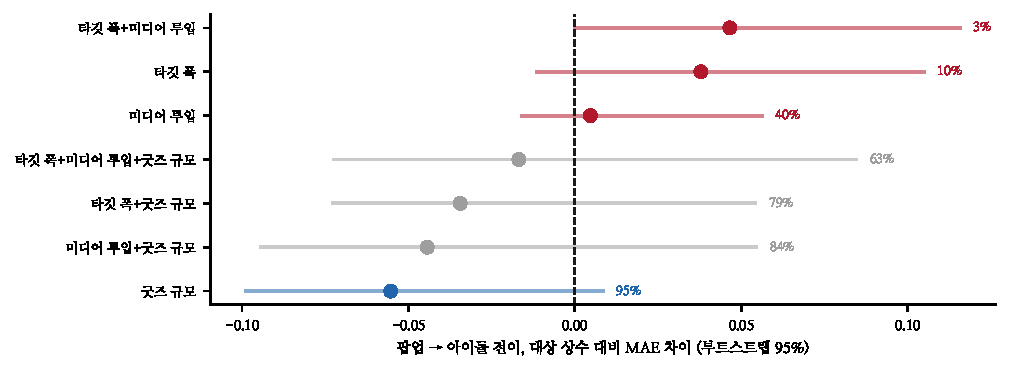
\includegraphics[width=\textwidth]{figs/subsets.pdf}
\caption{팝업 $\to$ 아이돌 전이, 축 조합별. 굿즈 규모 단독이 가장 강하고,
축을 더할수록 흐려진다. 막대는 부트스트랩 95\% 구간, 오른쪽 숫자는 이긴 비율.}
\end{figure}

\begin{table}[t]
\centering\tsize
\caption{팝업 $\to$ 아이돌. 축 조합별 부트스트랩 결과.}
\begin{tabular}{lrr}
\toprule
축 조합 & 차이 중앙 & 이긴 비율 \\
\midrule
\textbf{굿즈 규모} & \textbf{$-$0.0583} & \textbf{94\%} \\
미디어 $+$ 굿즈 & $-$0.0472 & 83\% \\
타깃 폭 $+$ 굿즈 & $-$0.0376 & 79\% \\
세 축 전부 & $-$0.0219 & 64\% \\
미디어 투입 & $+$0.0060 & 39\% \\
타깃 폭 & $+$0.0379 & 10\% \\
타깃 폭 $+$ 미디어 & $+$0.0492 & 2\% \\
\bottomrule
\end{tabular}
\end{table}

굿즈 규모 하나가 전부를 하고 있다. 다른 축을 더할 때마다 성적이 단조로 떨어진다.
타깃 폭은 단독으로 이긴 비율이 10\%이므로 넣으면 잡음만 추가된다.

\section{순열 검정 --- 첫 유의한 전이}

굿즈 규모 단독에 대해 직접 물었다. 팝업 계수가 아이돌에 대해 아무 정보도 담고 있지
않다면, 관측된 성적이 우연히 나올 확률은 얼마인가. 팝업 라벨을 4,000회 섞어
귀무 분포를 만들었다.

\begin{figure}[t]
\centering
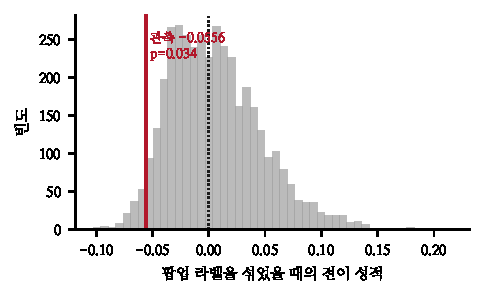
\includegraphics[width=\columnwidth]{figs/perm.pdf}
\caption{팝업 라벨을 섞었을 때의 전이 성적 분포와 실제 관측값. 4,000회 중
3.4\%만이 관측값 이하다.}
\end{figure}

\begin{table}[t]
\centering\tsize
\caption{굿즈 규모 단독, 팝업 $\to$ 아이돌. 아이돌 라벨은 학습에 쓰지 않았다.}
\begin{tabular}{lr}
\toprule
관측 차이 & $-$0.0556 \\
팝업 계수 & $+$0.213 \\
부트스트랩 (2,000회) 중앙 & $-$0.0543 \\
\hspace{1em}95\% 구간 & [$-$0.0990, $+$0.0096] \\
\hspace{1em}이긴 비율 & 95\% \\
순열 귀무 중앙 (4,000회) & $+$0.0019 \\
\textbf{순열 p} & \textbf{0.034} \\
\bottomrule
\end{tabular}
\end{table}

두 검정이 서로 다른 것을 말한다. 부트스트랩 구간은 0을 아슬아슬하게 넘고
($+$0.0096), 순열 검정은 p=0.034로 유의하다. 모순이 아니다 --- 부트스트랩은
\emph{효과 크기의 추정 정밀도}를 재고, 순열은 \emph{전이가 없다는 귀무가설}을
직접 검정한다. 우리가 묻는 것은 후자다. 효과 크기는 아직 정밀하지 않지만,
전이가 없다고 보기는 어렵다.

\claimx{팝업에서 사람이 매긴 굿즈 규모 축의 계수가 아이돌 초동 예측에 실제로
정보를 담고 있다. 이 프로젝트 최초의 도메인 간 전이다 (순열 p=0.034).}{독립적으로
수집한 새 아이돌 표본에서 같은 계수를 적용해 p가 0.05를 넘으면 이 결과는
표본 특수한 것이다.}

\section{그런데 되돌아오지 못한다}

같은 축, 반대 방향으로 보내면 실패한다.

\begin{figure}[t]
\centering
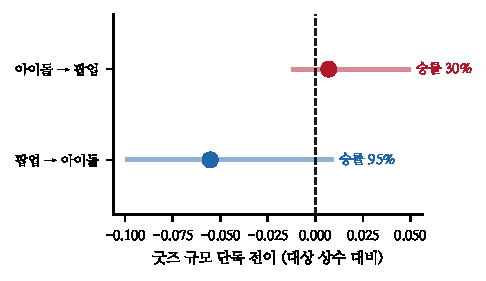
\includegraphics[width=\columnwidth]{figs/asym.pdf}
\caption{굿즈 규모 단독 전이의 비대칭. 한 방향은 되고 반대 방향은 되지 않는다.}
\end{figure}

\begin{table}[t]
\centering\tsize
\caption{굿즈 규모 단독, 양방향.}
\begin{tabular}{lrr}
\toprule
방향 & 부트 중앙 & 이긴 비율 \\
\midrule
팝업 $\to$ 아이돌 & $-$0.0543 & 95\% \\
아이돌 $\to$ 팝업 & $+$0.0070 & 29\% \\
\bottomrule
\end{tabular}
\end{table}

축이 도메인 불변이라면 방향은 상관없어야 한다. 그런데 상관있다.

설명은 측정 품질에 있다. 팝업의 굿즈 규모는 \emph{사람이 문서를 읽고 매긴 0--4
서수}다. 아이돌의 굿즈 규모는 \emph{상품 제목에서 규칙으로 뽑은 버전 수와 정가}다.
후자의 신뢰도는 재지 않았지만 전자보다 낮다고 보는 것이 자연스럽다.

노트 9는 축 측정 신뢰도가 0.79 아래면 축이 실용적 가치를 잃는다고 보고했다. 같은
논리가 전이에도 적용된다 --- 계수를 추정하는 쪽의 축이 잘 측정돼 있어야 그 계수가
옮길 값어치가 있다. 잘 측정된 쪽에서 못 측정된 쪽으로는 가고, 반대로는 못 간다.

\claimx{도메인 간 전이는 방향이 있으며, 그 방향은 축 측정 신뢰도가 높은 쪽에서
낮은 쪽이다.}{아이돌 축을 사람 태깅으로 다시 매겨 신뢰도를 올렸는데도 아이돌
$\to$ 팝업이 실패하면 원인은 측정 품질이 아니라 다른 것이다.}

\section{그래서 파운데이션 모델의 첫 슬롯}

열 편의 노트 끝에 확실한 것 하나가 남았다.

\begin{quote}\fontsize{9.5}{11.5}\selectfont
\textbf{굿즈 규모} --- ``닿으면 무엇을 얻는가'' --- 는 팝업과 아이돌에서 같은
방향으로 작동하며, 한 도메인에서 배운 계수가 다른 도메인에서 유의하게 쓰인다.
\end{quote}

이것이 파운데이션 월드모델의 첫 확정 슬롯이다. 팝업에서는 굿즈 종류 수로, 아이돌에서는
앨범 버전 수와 정가로 측정되지만 같은 것을 재고 있다.

미디어 투입은 부호는 맞으나 단독 전이가 39\%로 약하다. 후보로 남긴다. 타깃 폭은
현재 대리변수로는 무효이므로 재설계 대상이다.

\section{한계}

\begin{itemize}[leftmargin=1.1em,itemsep=0.15em]
\item 아이돌 축은 여전히 규칙 기반 유도다. 신뢰도를 재지 않았고, 비대칭 설명은
      그 신뢰도 차이를 가정하고 있으나 직접 측정한 것이 아니다.
\item 부분집합을 일곱 개 전부 돌리고 가장 좋은 것을 보고하므로 선택 편향이 있다.
      순열 p=0.034는 그 편향을 보정하지 않은 값이며, 일곱 조합에 본페로니를 적용하면
      0.24가 된다. 다만 굿즈 규모는 사후에 고른 것이 아니라 노트 9에서 부호가
      일치한 두 축 중 하나로 미리 지목돼 있었다.
\item 입장 허들 축은 지금 비어 있다. 다섯 축 중 셋으로만 검정하고 있다.
\item 아이돌 완전 케이스 63~69건, 팝업 75건. 양쪽 다 작다.
\end{itemize}

\section{다음}

\begin{enumerate}[leftmargin=1.3em,itemsep=0.15em]
\item 아이돌 굿즈 규모를 사람 태깅으로 다시 매기고 신뢰도 측정 --- 비대칭 설명의
      직접 검정.
\item 타깃 폭 대리변수 재설계. 인원 수가 아니라 데뷔 시점 팬덤 도달 범위 쪽에서 찾는다.
\item 입장 허들의 아이돌 대응물 수집 --- 팬클럽 가입비, 예약 경쟁 구조.
\item 세 번째 도메인 확보. 두 도메인으로는 ``불변''을 말하기 이르다.
\end{enumerate}

\vspace{0.6em}
\hrule height 0.3pt
\vspace{0.5em}
{\footnotesize
\textbf{참고문헌}\\[0.3em]
Ben-David, S. et al. (2010). A theory of learning from different domains.
\emph{Machine Learning}, 79(1--2), 151--175.\\[0.15em]
Carroll, R. J. et al. (2006). \emph{Measurement Error in Nonlinear Models},
2nd ed. Chapman \& Hall.\\[0.15em]
Good, P. (2005). \emph{Permutation, Parametric, and Bootstrap Tests of Hypotheses},
3rd ed. Springer.\\[0.15em]
Standley, T. et al. (2020). Which tasks should be learned together in multi-task
learning? \emph{ICML 2020}, 9120--9132.
}

\end{document}
